\documentclass[runningheads]{llncs}

\usepackage[T1]{fontenc}
\usepackage{amsmath,amssymb}
\usepackage{booktabs}
\usepackage{graphicx}
\usepackage{microtype}
\usepackage{url}
\setlength{\emergencystretch}{1.5em}

\newcommand{\method}{phase-pair holographic inversion}
\newcommand{\ms}{MS-SSIM}

\begin{document}

\title{Phase-Pair Holographic Inversion for Scanner-Equivalent OCT Digital Phantom Synthesis}
\titlerunning{Phase-Pair Holographic Inversion for OCT Phantoms}

\author{Anonymous Authors}
\authorrunning{Anonymous Authors}
\institute{Anonymous Institution}

\maketitle

\begin{abstract}
Generating a digital optical coherence tomography (OCT) phantom from a target
B-scan is a constrained coherent inverse problem: 300,000 nonnegative
scatterers must reproduce a log-compressed magnitude image after virtual
scanning. We present \method, a deterministic, training-free method. A
factorized axial--lateral scanner model is inverted with Tikhonov
regularization inside momentum alternating projections, which select a
scanner-feasible field phase while preserving the measured magnitude. Each
complex voxel coefficient is represented by two nonnegative scatterers at
carrier-equivalent depths. Their phasors match the coefficient at the center
wavenumber and their amplitude-weighted depth offset is zero, canceling the
first-order phase slope across the scanner bandwidth. A $256\!\times\!512$
scan uses 262,144 active scatterers and 37,856 zero-energy fillers. Across 120
public skin OCT scans rendered by the hosted challenge scanner, the method
achieved mean structural \ms{} 0.9943, median \ms{} 0.9946, and median LPIPS
0.0226. In source-equivalent evaluation, the complete configuration improved
mean structural \ms{} from 0.9559 for an earlier zero-phase,
single-scatterer configuration to 0.9946 and improved every filename-defined
acquisition series. Mean phantom generation time was 8.43 s (maximum 19.28 s),
well below the 600 s limit. These results establish scanner-equivalent image
fidelity, not unique recovery of biological microstructure; hidden-test
evaluation remains pending.

\keywords{Optical coherence tomography \and Digital phantom \and Phase retrieval
\and Coherent inverse problem \and Physics-based synthesis.}
\end{abstract}

\section{Introduction}

Optical coherence tomography (OCT) forms depth-resolved images from coherent
interference rather than direct observation of tissue reflectivity
\cite{huang1991oct}. This physics is useful for synthetic data generation:
given a spatial distribution of scatterers and scanner parameters, a virtual
scanner can produce an OCT B-scan. The reverse direction is substantially more
difficult. A displayed B-scan supplies a quantized, log-compressed field
magnitude but not the complex field phase, and many scatterer distributions
can produce nearly the same image.

The SynthOCT 2026 task makes the inverse direction concrete
\cite{matveev2026challenge}. For every supplied $256\!\times\!512$ skin B-scan,
a method must emit exactly 300,000 rows of $(x,y,z,E)$ scatterers. The fixed
virtual scanner then renders the phantom, and the render is compared with the
target. A practical solution must therefore satisfy two different criteria:
the file must obey a strict numerical contract, and its coherent field must
remain accurate after scanning. Treating each image pixel as an independent
positive reflector meets the first requirement but discards phase. Conversely,
an arbitrary complex inverse generally cannot be serialized because the file
format permits only nonnegative energy.

We address both constraints with \method. First, momentum alternating
projections choose an unobserved phase whose complex field lies near the range
of a regularized scanner. Second, every complex coefficient is encoded by two
nonnegative scatterers at depths that are phase-equivalent at the carrier.
Their weights preserve the desired coefficient while canceling its first
depth moment. The construction therefore removes the first-order spectral
phase error created by a single depth-shifted scatterer.

Our contributions are: (i) a separable coherent inverse in which phase is
selected jointly with regularized scanner inversion; (ii) an analytic
two-scatterer code for nonnegative serialization of complex coefficients; and
(iii) a fail-closed evaluation and submission pipeline, including all 120
hosted-scanner renders and an explicit separation between organizer-compatible
derived maps and scientifically calibrated float maps. We deliberately claim
\emph{scanner equivalence}: magnitude-only input is insufficient to identify a
unique biological microstructure.

\section{Related Work}

Physics-based OCT simulation has been used for controlled algorithm evaluation
and data augmentation \cite{sovetsky2025simulation}. More recent work combines
tissue-mimicking phantoms with virtual scanning for few-shot model training
\cite{nikoshin2026phantoms}. These forward pipelines motivate digital phantom
generation, but the target-conditioned inverse considered here additionally
requires selecting a coherent phase and representing it with a constrained
scatterer list.

Alternating projection methods recover unobserved phase by switching between
measurement and object constraints \cite{gerchberg1972practical,fienup1982phase}.
Our setting differs from Fourier-magnitude phase retrieval: the forward model
is the specified OCT scanner, the output field magnitude is fixed at every
image pixel, and the object coefficients may be complex before serialization.
We use Tikhonov pseudoinverses \cite{tikhonov1963regularization} to prevent
poorly observed scanner modes from dominating. The phase-pair code is then a
closed-form physical output parameterization rather than an additional learned
decoder.

\section{Method}

\subsection{Target Magnitude and Coherent Scanner}

Let $S\in[0,1]^{N_z\times N_x}$ denote the displayed OCT scan. Dataset and
scanner metadata specify an approximately 51 dB display range
\cite{matveev2025dataset}. We invert the display compression to a normalized
field magnitude
\begin{equation}
  M = 10^{(51S-51)/20}.
  \label{eq:magnitude}
\end{equation}
The subtraction maps the brightest display value to unit field magnitude;
global amplitude is later chosen to satisfy the reflection-energy bound.

Under the challenge's low-reflectivity reference model, we write the complex
B-scan field as a separable linear operator
\begin{equation}
  \mathcal{P}(C)=A C L^{\mathsf T},
  \label{eq:forward}
\end{equation}
where $C\in\mathbb{C}^{N_z\times N_x}$ is a grid of complex voxel
coefficients. Columns of $A$ are axial responses formed from the inverse FFT of
the Hann-windowed scanner spectrum with two-way phase
$\exp(-2\mathrm{i}kz)$; $L$ contains Gaussian lateral beam responses,
truncated beyond three squared beam radii. The fixed geometry is
$N_z=256$, $N_x=512$, 6 $\mu$m axial/lateral sampling, 1.3 $\mu$m center
wavelength, and 10 $\mu$m beam radius.

For either operator $B\in\{A,L\}$ with singular value decomposition
$B=U\Sigma V^{*}$, the regularized inverse is
\begin{equation}
 B_{\alpha}^{+}=V\,\mathrm{diag}\!\left(
 \frac{\sigma_j}{\sigma_j^2+\alpha^2}\right)U^{*}.
 \label{eq:tikhonov}
\end{equation}
We fix $\alpha_A=0.02$ and $\alpha_L=0.05$ globally. No parameter is selected
per image.

\subsection{Momentum Phase Selection}

The target constrains $|F|=M$ but leaves $\arg F$ unobserved. Starting from
$F_0=M$, iteration $t$ alternates between the regularized coefficient space
and the scanner range:
\begin{align}
 C_t &= A_{\alpha_A}^{+}F_t(L_{\alpha_L}^{+})^{\mathsf T}, \\
 \widehat F_t &= A C_t L^{\mathsf T}. \label{eq:projection}
\end{align}
Let $q_t=\arg\widehat F_t$. Circular momentum extrapolates the phase without
changing the measured magnitude,
\begin{align}
 \Delta q_t &= \arg\exp\!\left[\mathrm{i}(q_t-q_{t-1})\right],\\
 F_{t+1} &= M\exp\!\left[\mathrm{i}(q_t+\beta\Delta q_t)\right].
 \label{eq:momentum}
\end{align}
We use 200 iterations and $\beta=1$. The final $C$ is recomputed from $F$.
This process selects one feasible representative from a non-unique inverse; it
does not reveal the phase of the acquired tissue field.

\begin{figure}[t]
  \centering
  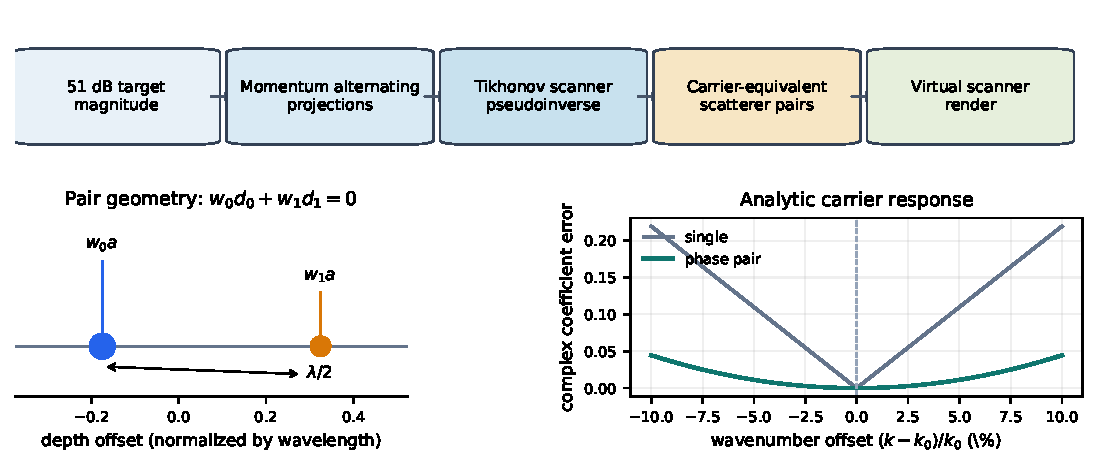
\includegraphics[width=\textwidth]{figures/method_overview.pdf}
  \caption{Method overview and phase-pair construction. The two scatterers are
  carrier-equivalent, while their weighted first depth moment is zero. The
  analytic response plot uses $\phi=0.7\pi$ only for illustration; all phases
  use the same closed-form construction.}
  \label{fig:method}
\end{figure}

\subsection{Nonnegative Phase-Pair Encoding}

Consider a coefficient $c=a\exp(\mathrm{i}\phi)$ at voxel center $z_c$.
Because the scanner applies two-way propagation, a scatterer at offset $d_0$
matches its phase at center wavelength $\lambda$ when
\begin{equation}
 d_0=-\frac{\phi\lambda}{4\pi}.
\end{equation}
A single shifted scatterer is exact only at the center wavenumber. We add a
carrier-equivalent companion
\begin{equation}
 d_1=d_0-\mathrm{sign}(d_0)\frac{\lambda}{2},
\end{equation}
where $\mathrm{sign}(0)$ is taken as $+1$. The half-wavelength separation
changes the two-way carrier phase by $2\pi$, so both phasors are aligned at
$k_0=2\pi/\lambda$. Nonnegative weights
\begin{equation}
 w_0=\frac{-d_1}{d_0-d_1},\qquad
 w_1=\frac{d_0}{d_0-d_1}
 \label{eq:weights}
\end{equation}
satisfy $w_0+w_1=1$ and $w_0d_0+w_1d_1=0$. Thus
\begin{equation}
 H(k)=a\sum_{j=0}^{1}w_j\exp(-2\mathrm{i}kd_j)
\end{equation}
equals $c$ at $k_0$, and its first-order phase perturbation about $k_0$
vanishes. Figure~\ref{fig:method} contrasts this quadratic local error with the
linear error of a single shifted scatterer.

All amplitudes are globally scaled so the maximum reflection amplitude is
$10^{-3}$; the serialized energy is $E_j=100(sw_ja)^2$ percent, whose maximum
is $10^{-4}\%$. Two rows for every voxel yield
$2(256)(512)=262{,}144$ active scatterers. We append 37,856 deterministic
zero-energy rows to reach exactly 300,000. Active rows use $y=0$; filler rows
remain within the 10 $\mu$m beam-radius bound. Serialization uses finite
numeric values and checks every coordinate and energy bound before writing.

\section{Experimental Design}

\subsection{Data, Scanner, and Pairing Controls}

We use the public CC BY 4.0 in-vivo skin OCT set
\cite{matveev2025dataset,sovetsky2026skin}: 120 uint8 B-scans at
$256\!\times\!512$, balanced across sex, age group, and cheek/eye-corner site.
Filenames form 40 acquisition series with three frames (50, 250, and 450).
They should not be interpreted as 120 confirmed independent subjects. All
reported hosted results use the challenge API. For each case, we retain the
reference-relative path, flattened phantom name, request identifier, raw PNG,
grayscale PNG, configuration, timings, and SHA-256 hashes. Inventory checks
verified a one-to-one set of 120 references, phantoms, raw renders, grayscale
renders, and metric rows; raw-to-grayscale conversion was exact for all cases.

The primary image metrics are \ms{} \cite{wang2003msssim} and AlexNet LPIPS
\cite{zhang2018lpips}. The hosted development set is descriptive evidence, not
an organizer-issued score. Local source-equivalent rendering is used only to
compare fixed configurations and timing. Paired inference groups the three
frames by filename-defined series: we bootstrap 40 series means (200,000
replicates, fixed seed) and use a one-sided exact Wilcoxon signed-rank test.

\subsection{The 40 dB/51 dB Evaluation Contradiction}

The dataset and scanner document approximately 51 dB, which we use in
Eq.~\ref{eq:magnitude}. The public Part3 map processor instead linearizes PNGs
with 40 dB. It also normalizes the reference and prediction optical attenuation
coefficient (OAC) independently, forces an invalid terminal OAC estimator row
to white, duplicates speckle-map edge pixels, clips SC/RSC displays, and lets
Matplotlib autoscale some already-normalized RSC PNGs. Consequently, the
``reference'' OAC/SC/RSC files are organizer-defined transformations of the
reference B-scan, not independently measured ground-truth parameter maps.

We therefore maintain two disjoint modes. \texttt{organizer-compatible-v1}
freezes the published 40 dB behavior byte-for-byte, including save-time
autoscaling, and is used only for competition-formula estimates.
\texttt{scientific-v1} uses 51 dB float maps, fixed display scales, a
reference-defined signal-support mask, denominator reliability, explicit
filter-footprint masks, and propagation of invalid OAC pixels into RSC
validity. Mode-specific directories prevent cross-mode overwrites. LPIPS and
the competition formula are rejected for scientific float maps. This decision
preserves organizer reproducibility without letting a known display encoding
define the physical inverse.

\subsection{Configurations and Submission Integrity}

We compare an earlier zero-phase, single-scatterer configuration; the complete
phase-pair method with 50 iterations; and the final method with 200 iterations.
This is a configuration comparison, not a factorial ablation: regularization,
phase selection, encoding, and evaluator precision are not all independently
controlled. Causal attribution to one component would require a fixed-
regularization $2\!\times\!2$ phase/encoding study.

For preliminary delivery, 60 cases are deterministically selected with seed
2026 and joint sex--age--site balancing (30/30 along every marginal; 7 or 8 per
joint stratum). Before atomic ZIP publication, every member is reparsed and
checked for exactly $300{,}000\!\times\!4$ finite values, scanner bounds,
root-flat naming, case-insensitive uniqueness, source/reference hashes, CRC,
and content hashes. The final archive is then independently reparsed against
its manifest. This procedure tests transport integrity; it cannot replace the
submission portal's own schema validation.

\section{Results}

\begin{table}[t]
\caption{Source-equivalent public-set comparison. Values describe complete
configurations; they do not isolate the effect of phase pairing. Runtime is
phantom generation only.}
\label{tab:local}
\centering
\small
\begin{tabular}{lrrrrrr}
\toprule
Configuration & Iter. & Mean & Median & Min. & Mean s & Max s\\
\midrule
Zero phase, single scatterer & 0 & 0.955954 & 0.956021 & 0.933827 & 0.583 & 3.873\\
Phase pair & 50 & 0.993518 & 0.993899 & 0.984114 & 2.984 & 5.963\\
Phase pair & 200 & \textbf{0.994588} & \textbf{0.994849} & \textbf{0.985133} & 8.427 & 19.279\\
\bottomrule
\end{tabular}
\end{table}

Table~\ref{tab:local} shows that the complete 200-iteration method increases
mean source-equivalent structural \ms{} by 0.03863 over the earlier
configuration and reduces the mean distance to one by 87.7\%. All 40
filename-defined series improve. The cluster-bootstrap 95\% interval for the
mean gain is $[0.03753,0.03979]$; the one-sided exact signed-rank test gives
$p=9.1\times10^{-13}$. Increasing phase iterations from 50 to 200 improves all
120 images by a mean 0.00107. The mean generation time is 8.43 s, the median is
7.96 s, and the maximum is 19.28 s, leaving at least 580 s of the 600 s limit.

\begin{table}[t]
\caption{All-120 hosted-scanner results. Asterisks mark organizer-compatible
derived views, not calibrated physical ground truth. The composite is a local
public-development estimate, not an official or hidden-test score.}
\label{tab:hosted}
\centering
\small
\begin{tabular}{lrrrr}
\toprule
View & \ms{} mean & \ms{} median & LPIPS mean & LPIPS median\\
\midrule
Structural & 0.994284 & 0.994553 & 0.022432 & 0.022611\\
OAC$^{*}$ & 0.999648 & 0.999657 & 0.001116 & 0.001057\\
SC$^{*}$ & 0.998012 & 0.998173 & 0.008392 & 0.007857\\
RSC$^{*}$ & 0.998172 & 0.998306 & 0.007389 & 0.006533\\
\midrule
\multicolumn{4}{l}{Eight-term organizer-compatible estimate} & 0.994079\\
\bottomrule
\end{tabular}
\end{table}

Hosted-scanner structural results remain close to the source-equivalent
results (Table~\ref{tab:hosted}). The minimum hosted structural \ms{} is
0.98570 and the maximum is 0.99828. The organizer-compatible derived views are
numerically higher, but their shared transformations, clipped backgrounds, and
encoding defects make them unsuitable evidence of quantitative optical-
property recovery. We report them only because they enter the published
development formula.

\begin{figure}[t]
  \centering
  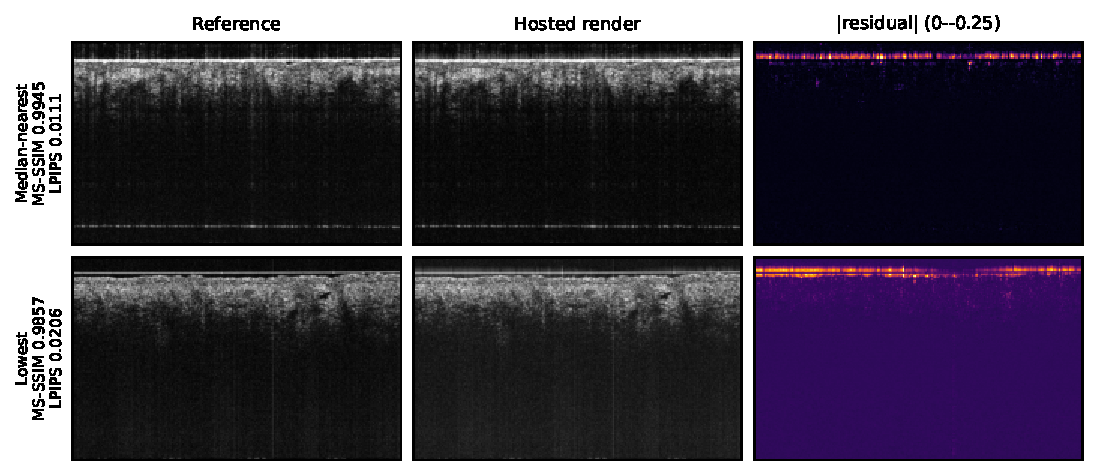
\includegraphics[width=\textwidth]{figures/qualitative.pdf}
  \caption{Hosted-scanner examples selected by a predeclared rule: the sample
  nearest the median structural \ms{} and the lowest-scoring sample. Residuals
  use a common 0--0.25 display range. The lowest-scoring case retains the main
  interfaces but shows larger low-amplitude texture differences.}
  \label{fig:qualitative}
\end{figure}

Figure~\ref{fig:qualitative} shows the median-nearest and lowest hosted cases.
The method reproduces layer geometry and most speckle-scale organization. The
residual is largest in low-amplitude texture and near bright interfaces, which
is consistent with regularized suppression of poorly observed modes and with
the fact that only magnitude is constrained.

\section{Discussion}

The central result is that a constrained nonnegative scatterer file can encode
a complex inverse accurately enough to survive an external coherent scanner.
Alternating projections exploit the phase freedom of a magnitude image, and
the phase pair transfers the selected coefficient into a legal physical
parameterization. The method is deterministic, has no training set or learned
weights, and uses one global parameter set.

Several boundaries are essential. First, scanner equivalence is not biological
identification. Magnitude-only OCT does not uniquely determine scatterer
positions, so the zero-energy fillers and sub-wavelength phase offsets should
not be interpreted as histology. The low-reflectivity linear model and known
scanner parameters are also assumptions; a scanner with different spectrum,
sampling, or beam profile requires new operators. Second, the public set is a
development corpus with correlated frames. The cluster analysis mitigates but
does not eliminate this limitation, and hidden-test performance is unknown.
Third, the current configuration comparison does not isolate momentum phase
selection from phase-pair encoding. A factorial study with fixed
regularization is the most important missing ablation.

The feature-map audit explains why the visually unusual ``reference'' maps
cannot validate tissue properties. OAC, SC, and RSC are computed from the same
8-bit reference image using estimator, padding, clipping, normalization, and
save rules; no separate parametric annotation enters. Independent reference
normalization can even make unequal physical ranges look similar. Our dual-mode
implementation prevents these quirks from contaminating the 51 dB inversion,
while retaining an exact compatibility path for transparent comparison. A
future physical study should use calibrated raw intensities, independently
measured optical properties, and uncertainty-aware regions of validity.

Finally, deterministic archive validation reduces operational failure but does
not establish scientific validity. The 60-case preliminary subset is balanced
for the labels exposed in the public directory, not for unobserved participant
identity or tissue pathology. Portal acceptance and the final organizer score
remain external checks.

\section{Conclusion}

We introduced \method{} for target-conditioned OCT digital phantoms. A
regularized coherent inverse selects a scanner-feasible phase, and an analytic
two-scatterer code preserves each complex coefficient while canceling its
first-order spectral phase slope. All-120 hosted renders show high structural
fidelity within a strict 300,000-row and 600 s contract. The method should be
understood as scanner-equivalent synthesis; biological microstructure recovery
and hidden-set generalization remain open evaluations.

\begin{credits}
\subsubsection{Acknowledgements} Omitted for double-blind review.
\subsubsection{Use of Generative AI} Generative AI tools were used in the
preparation of this work. GPT-5.6 Sol (OpenAI) supported methodology
development, programming, and manuscript writing, and Claude Science Opus~4.8
(Anthropic) was used for manuscript revision. The authors reviewed and verified
all AI-assisted text, code, and analysis, and take full responsibility for the
content of this paper in accordance with the MICCAI policy on the use of large
language models.
\subsubsection{Disclosure of Interests} The authors have no competing interests
to declare that are relevant to the content of this article.
\end{credits}

\bibliographystyle{splncs04}
\bibliography{references}

\end{document}
